
\chapter{Experiments, Results and Analysis}
\label{experiments}
\epigraph{Experiment is the sole judge of scientific ``truth''}
{\textit{The Feynman Lectures on Physics, Introduction, Richard Feynman, 1961.}}
The previous chapters have described the models and the implementation used to simulate CSE.
The \usermodel model is used to create CUDF* documents given the probabilities a user will request to upgrade and install components, 
and the criteria used to accomplish these requests.
These documents describe the evolution of an Ubuntu system for a year starting on October 30th 2009.
Given such a document, the implementation GJSolver can be used to resolve the exact evolution of the system.
This process of describing a user in \usermodel, generating CUDF* documents, then resolving the evolution is used to explore CSE.

This chapter presents experiments and results to study the effects of CSE.
The specific effects that are focused on are the change made to the system, and the out-of-dateness of the system during evolution.
This exploration is accomplished through trying to answer the questions:
\begin{enumerate}
  \item What effects do the probabilities user upgrades per day ($u$) and a user installs a component per day ($i$) have during CSE?
  \item Can the upgrade criteria ($U$) be altered to decrease out-of-dateness?
  \item Can the upgrade criteria ($U$) be altered to reduce change?
  \item What are the effects of these new criteria when simulating ``real'' users?
\end{enumerate}
This chapter is organised to present these questions in this order. 

\section{Upgrade and Install Variable Analysis}
How often a user decides to upgrade their system or install a component will effect how the system evolves.
This section attempts to quantify the effects on change and out-of-dateness that these actions have on the users systems.

These experiments simulates users altering the probabilities a user will install a component $i$ and upgrade their system $u$,.
The criteria to install $I$ and upgrade $U$ are defaulted to the ones used by \texttt{apt-get}. 
\texttt{apt-get}'s $U$ criteria is \texttt{-removed,-new,-uptodatedistance}, and $I$ criteria is \texttt{-ovpp,-removed,-changed,-uptodatedistance} as described in section \ref{impl.validation} 

\subsection{Boundary Cases}
The first experiments assign values to the variables in \usermodel that describe the boundary cases for $i$ and $u$:
\begin{table}[h!]
\centering
\begin{tabular}{|l | c | c | c }
\hline
User Name 				 	& \# generated 	& $u$ 		& $i$ 			\\ \hline
Always Upgrade				& 1 			&1			& 0				 \\
Control						& 1 			& 0			& 0				\\
Always Install 				& 30 			& 0			& 1				 \\
Always Upgrade\&Install 	& 30 			&1			& 1				\\
\end{tabular}
\caption{Users that are the boundary cases in the simulation.}
\label{exp.extremeusers}
\end{table}
This table also states the number of simulations that were run for each user, i.e. the ``Always Install'' user had 30 CUDF* documents created and resolved.
The number of simulations run for a user is a trade-off between time to complete the simulations and accuracy of results.
The number of simulations run is based on the randomness of the simulated users (as described in section \ref{sim.randomness}) 
as well as the experience gained when developing the simulation as to the variability of the results.

\subsubsection{Results and Analysis}
First, how out-of-date these simulated systems become will be explored.
This out-of-dateness is measured using the function up-to-date distance (UTTD) function, as described in section \ref{impl.criteria}.
This measurement is the number of components that are a greater version than a component currently installed.
A problem that exists with this measurement is that it does not take into account the size of a system.
As a system grow the UTTD will grow as there will be more components that become out of date.
To normalise this effect the measurement UTTD per component (UTTDpC) is defined as the UTTD per installed component.
The UTTDpC of each simulated system is presented in figure \ref{exp.q1auttdpc}.
\begin{figure}[htp]
\begin{center}
  \includegraphics[width=\textwidth]{plots/q1auttdperc}
  \caption{The Up-to-date distance per Component (UTTDpC) of the simulated systems.}
  \label{exp.q1auttdpc}
\end{center}
\end{figure}

This figure shows that all systems slowly become out-of-date.
However, users that do not upgrade, the ``Control'' and ``Always Install'' users, become nearly three times more out-of-date than ones that upgrade every day.
The speed at which systems become out-of-date increases over the months between March and May 2010.
The reason for this is likely due to the increased development effort because of the Ubuntu 10.04 release in April 2010.
The users that upgrade are less affected by this release as they are continually upgrading to the new component versions.

This figure also shows the effect of the normalisation, where the install variable $i$ has little effect on the UTTDpC of a component system.

Second, how much change each simulated system went through during evolution is measured.
To measure change the ``change'' function as described in section \ref{impl.criteria} is used.
The total change, i.e. the sum of all change a system has to a date, is presented in figure \ref{exp.q1achange}
\begin{figure}[htp]
\begin{center}
  \includegraphics[width=\textwidth]{plots/q1achange}
  \caption{The total change of the simulated systems.}
  \label{exp.q1achange}
\end{center}
\end{figure}

As is expected, this figure shows that if a user upgrades their system changes more during the release of Ubuntu 10.04.
During the months March, April and May of 2010 had a mean of 266 changes per month for the ``Always Upgrade'' user.
All other months had had a mean of 105 changes per month, showing a more than 250\% increase in change over the release months.
This is likely because the increased development of components leads to an increased release of versions that have to be upgraded.
This increased change cannot be seen in the ``Always Install'' users as they will not change in response to newer versions.

The ``Always Install'' users start by changing their systems quickly, then after a month this change slows to a constant rate.
This can be seen with the mean change per day, during the first month it is 4.9, where the final 11 months it is 3.0.
After a small investigation this reduction in change can be explained due to the common reuse of individual components e.g. \texttt{libaudio2} and \texttt{libqt3-mt}.
Many components require such components to be installed, they are then required to be installed in the first month.
After this installation they are no longer required to be added, so the future change is reduced. 
These effects described here may be due to the way in which \usermodel selects components to be installed.

The ``Always Upgrade\&Install'' users changes more than the combined amount of ``Always Upgrade'' and ``Always Install'' changes.
The mean total change of the ``Always Upgrade'' user is 1655, the ``Always Install'' user is 1137 and the ``Always Upgrade\&Install'' user is 3482.
This shows that a user that always upgrades and installs changes more than 700 components more than the sum of just installing and just upgrading.
The additional change is due to the installed components increasing the amount of components to be upgraded.

\subsection{Failures}
These initial experiments are the most extreme users that can be simulated.
This means phenomena that occur rarely are most observable in these simulations.
For this reason, these simulations were chosen to be closely inspected for various failures.

Three types of failure were observed in the results of these simulations:
\begin{enumerate}
  \item \textbf{Hard Failure}: Where a request has no satisfactory solution, therefore no change is made to the system.
  \item \textbf{Soft Failure}: To satisfy an install request a significant amount of components must be removed.
  \item \textbf{Multi-component Failure}: A type of hard failure where multiple components must be installed to satisfy a request. 
  This causes the next upgrade request to fail and the next install request to remove the offending components.
\end{enumerate}

%%%Hard failures
Hard failures where observed to occur in 24 of the 60 ``Always Install'' and ``Always Upgrade\&Install'' users, and never in the ``Always Upgrade'' user.
Only 40 total failed requests occurred over these 24 simulated users.
All these hard failures, except those that are multi-component failures, were failed install requests.
Given each ``Always Install'' user has 365 requests and each ``Always Upgrade\&Install" user has 730 requests, 
and 30 users of each type were simulated, the chance for a request to fail is just over 0.12\%.
This means the chance for a hard failure to occur is extremely low in this simulation.

Due to the difficultly of finding the constraints that caused these failures \citep{quickxplain},
and the rarity of these failures, the specific reasons for hard failures are not further explored.

%%%Soft Failure TODO
Soft failures are called ``soft'' because the request that causes them succeeds, however does so at the detriment to the system.
They are defined to cause more than 100 components in the system to be removed in order to satisfy the install request.
Eight soft failures were observed in eight different ``Always Install'' and ``Always Upgrade\&Install'' users.
There are three interesting points that were observed with these failures:
\begin{enumerate}
  \item seven of the soft failures occurred during the Ubuntu 10.04 release month of April 2010.
  \item the component that caused the soft failure is removed five times in the following days.
  \item Each request reached the time limit allowed by GJSolver, and was interrupted. 
\end{enumerate}
This leads to the conclusion that soft-failures occur because of the increased component evolution caused by the Ubuntu release cycle which creates difficult to optimise problems.
The effect of these soft failures can be seen in figure \ref{exp.q1achange} 
where the standard deviation of change for both ``Always Install'' and ``Always Upgrade\&Install'' users increases after the Ubuntu 10.04 release.
Given that only 8 soft failures occurred of all the requests, this problem is seen as minor.
Although, in future experiments the detection of soft failures may lead to more accurate analysis. 

%%%The multi component fialure
An interesting failure occurred when the situation arose that installing the package \texttt{chromium-browser} required two versions of the package \texttt{libc6} to be installed. 
This lead to the following upgrade request to fail, and the following install request to remove \texttt{chromium-browser} and upgrade to the newest version of \texttt{libc6}.
This instance, although rare, shows the case that at some points the hard constraint that Debian has to have only one version of each component installed,
can restrict the user.

%%%Disclaimer
All these failures are directly caused by, or are a result of an install request.
Given the selection of components is the most random part of the simulation, the failures and/or the rates they occur may directly be a product of this randomness.
This was discussed in section \ref{sim.modelvalidation}.


\section{Decreased Out-of-dateness During Evolution}
In the previous section the criteria used during evolution were the criteria used by \texttt{apt-get}.
In this section, this criteria is altered to attempt to reduce the out-of-dateness of the system during evolution.


\section{Reduction of Change During Evolution}

\subsection{Stable Version}
%%%Here is a real example of this happening
An example of this described situation is show in figures \ref{apachelog} and \ref{apachebug}.

\begin{figure}[htp]
\begin{center}
\begin{alltt}
apache2 (2.2.20-1) unstable; urgency=low

  * New upstream release.
  * Fix some regressions related to Range requests caused by the CVE-2011-3192
    fix. Closes: #639825
\ldots

 -- Stefan Fritsch <sf@debian.org>  Sun, 04 Sep 2011 21:50:22 +0200

apache2 (2.2.19-2) unstable; urgency=high

\ldots

 -- Stefan Fritsch <sf@debian.org>  Mon, 29 Aug 2011 17:08:17 +0200
\end{alltt}
\caption[Apache Changelog]{An extract from the apache changelog located on http://changelogs.ubuntu.com/}
\label{apachelog}
\end{center}
\end{figure}

\begin{figure}[htp]
\begin{center}
\begin{alltt}

Reported by: Takis Issaris <takis.issaris@uhasselt.be>
Date: Tue, 30 Aug 2011 16:09:01 UTC
Severity: important
Found in versions 2.2.9-10+lenny10, 2.2.16-6+squeeze2, apache2/2.2.19-2

\ldots

Package: apache2.2-common
Version: 2.2.9-10+lenny10

Yesterday evenings update broke our Apache server setup,
\ldots
\end{alltt}
\caption[Apache Bug Report]{Extract from the bug report \#639825, filed with Debian}
\label{apachebug}
\end{center}
\end{figure}

A summary of these events are:
\begin{enumerate}
  \item Apache developer Stefan Fritsch released a new version of their server, apache2/2.2.19-2, on 29 Aug 2011.
  \item Takis Issaris upgraded to this version which broke his system on 29 Aug 2011.
  \item Takis Issaris submits a bug report on 30 Aug 2011, where he and Stefan Fritsch discuss the causes.
  \item On 04 Sep 2011 (5 days after the initial ug report) Stefan Fritsch releases a new version 2.2.20-1 that fixes this bug.
\end{enumerate}


\section{Real Evolution}
During the previous experiments how often the user upgrades or installs a component have been assigned values that may not be ``realistic''.
This section presents the final experiments where the variables are assigned values calculated from real user's systems.


%%%%%%%%%%%%%%%%%%%%%%%%%%%%%%%%%%%%
\subsubsection{Extracting Information from the User Submitted Logs}
These variables of update probability and user install probability can be extracted from the user submitted logs from the survey.
Initially, 31 logs where submitted, these logs were filtered to be APT logs, of more than 15 days long.
This resulted in 19 logs of between 23 and 277 days long to be processed.

An extract from one of these logs is shown in figure \ref{aptlog}.
\begin{figure}[htp]
\begin{center}
\begin{alltt}
\ldots
Start-Date: 2010-12-21 11:32:28
Install: libnet-daemon-perl (0.43-1), libhtml-template-perl (2.9-1), libdbi-perl (1.609-1build1), mysql-client-core-5.1 (5.1.41-3ubuntu12.8), libdbd-mysql-perl (4.012-1ubuntu1), mysql-server-5.1 (5.1.41-3ubuntu12.8), mysql-client-5.1 (5.1.41-3ubuntu12.8), libmysqlclient-dev (5.1.41-3ubuntu12.8), libplrpc-perl (0.2020-2), mysql-server-core-5.1 (5.1.41-3ubuntu12.8), mysql-server (5.1.41-3ubuntu12.8), libmysqlclient16-dev (5.1.41-3ubuntu12.8)
Upgrade: mysql-common (5.1.41-3ubuntu12.6, 5.1.41-3ubuntu12.8), libmysqlclient16 (5.1.41-3ubuntu12.6, 5.1.41-3ubuntu12.8)
End-Date: 2010-12-21 11:33:03
\ldots
\end{alltt}
\caption[APT log extract]{An extract of an APT log file}
\label{aptlog}
\end{center}
\end{figure}

These logs mainly describe the changes made to the system by APT, not necessarily what the user requested.
This is because APT may be used through another application, like semantic, to install or update the system.
As the criteria of APT is known, some information about the action the user requested can be inferred.

Given APT will never install or remove a component if the system is updated; 
if a package is upgraded but none are removed or installed then the user probably selected to update.
Also, if a package is installed, then the user requested a single package to be installed.
This second rule is assuming that only one package was selected, and not two at the same time.

Using these rules, each log is processed, and the variables of update probability and install distribution are measured.


\subsubsection{Measuring the Effect}
By calculating the difference in days between each version of all components in the repository, 
over the dates of the simulation how often this situation occurs, where packages are quickly updated, can be measured.
In figure \ref{comeponentversionreleases} a graph is presented measuring the time difference between version releases.
 
\begin{figure}[htp]
\begin{center}
  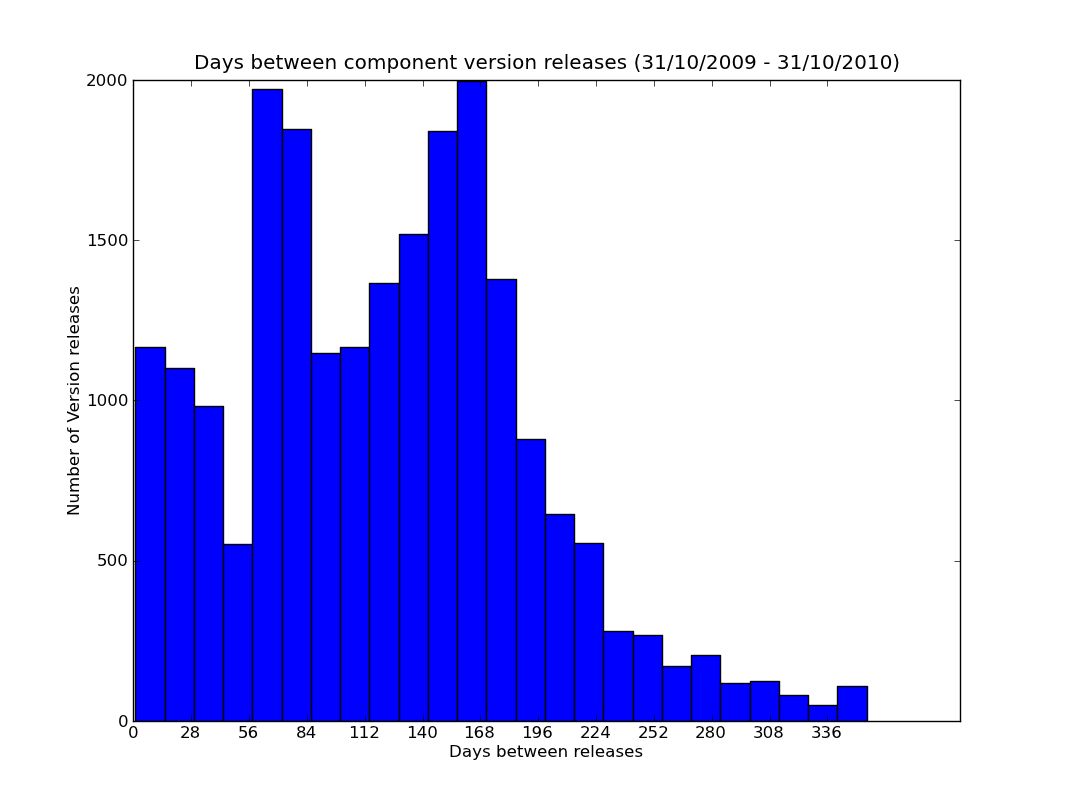
\includegraphics[width=\textwidth]{ubuntusimulationpics/versionreleasedistribution}
  \caption[labelInTOC]{Distribution of the releases of component versions between 31/10/2009 - 31/10/2010}
  \label{comeponentversionreleases}
\end{center}
\end{figure}

There are two points on this graph are noteworthy, firstly there is a large amount of components that release after 3 and 6 months.
Secondly there is a smaller but significant amount of components that have been released less than a month after the previous release.


\section{Summary}
%%%A list of the answers gained from the questions
